\documentclass[12pt,a4paper]{article}
\usepackage{tpl}
\usepackage{chessboard}
\dbegin{Кружок 7 класса, продолжающие, школа 179}{Решения занятия №15}

\z Оля и Аня живут в одном доме и выходят в школу вместе. Каждый шаг Оли на $10\%$ длиннее Аниного, но Оля делает в минуту на $10\%$ меньше шагов, чем Аня. Кто раньше придёт в школу?

\s Олин шаг в $\frac{11}{10}$ раз длиннее, но в минуту она делает $\frac{9}{10}$ от количества шагов Ани. Значит, за минуту она проходит $\frac{99}{100}$ от расстояния, проходимого Аней. Аня идёт быстрее и придёт раньше.\QEDA\\

\z Чему равна последняя цифра числа $2^{2019}$?

\s Последние цифры изменяются по циклу 2--4--8--6. У $2019$ остаток $3$ при делении на $4$, значит, $2^{2019}$ заканчивается на 8.\QEDA\\

\z На столе лежат четыре яблока весом 200г, 300г, 400г и 450г. Карлсон, а затем Малыш берут по яблоку и одновременно начинают есть их с одинаковой скоростью. Доевший берет следующее яблоко, каждый хочет съесть как можно больше. Какое яблоко выбрать Карлсону вначале?

\s Карлсон берёт яблоко в 300 граммов. К тому моменту, как он его доест, яблоко либо в 400 граммов, либо в 450 граммов будет свободно. С ним Карлсон набирает больше половины. Ответ находится перебором яблок.\QEDA\\

\z Леспромхоз решил вырубить сосновый лес, но экологи запротестовали. Тогда директор леспромхоза всех успокоил, сказав: <<В лесу $99\%$ сосен. Мы будем рубить только сосны. После порубки сосны будут составлять $98\%$ всех деревьев>>. Какую часть леса вырубит леспромхоз?

\s Изначально деревьев было в 100 раз больше, чем не-сосен, а стало в 50 раз больше, чем не-сосен. При этом количество не-сосен не изменилось. Ответ: половину леса.\QEDA\\

\z Петя заметил, что у всех его 25 одноклассников различное число друзей в этом классе. Сколько друзей в классе у Пети? (Найдите все решения).

\s Рассмотрим Васю --- одноклассника Пети, у которого больше всего друзей, и Колю --- одноклассника, у которого меньше всего друзей. Заметим, что либо у Коли 0 друзей, либо у Васи все ученики класса (кроме него самого) --- друзья. В обоих случаях Вася дружит с Петей, а Коля нет. Уберём из класса Васю и Колю. Все количества друзей у одноклассников Пети снова различны, у Пети теперь на 1 друга меньше, в классе на 2 человека меньше. Так можно сделать 12 раз, после чего останется Петя и ещё один человек. Они либо дружат, либо нет, причём оба варианта возможны. Ответ: 12 или 13.\QEDA\\

\z Какое наибольшее число слонов можно расставить на шахматной доске $8\times8$, чтобы они не били друг друга?

\s Пример на 14 слонов нарисован внизу \ref{bishops}. Докажем, что на клетках одного цвета не может быть 8 слонов. Действительно, есть 7 диагоналей, параллельных большой диагонали, и на каждой из них не более одного слона.\QEDA\\

\z Какое наибольшее число коней можно расставить на шахматной доске $8\times8$, чтобы они не били друг друга?

\s Пример на 32 коня --- все белые клетки. Больше нельзя, поскольку клетки доски можно разделить на пары, что между клетками в каждой паре можно пройти ходом коня.\QEDA\\

\z Из листа клетчатой бумаги размером $11\times11$ клеток вырезали по клеткам 15 квадратиков $2\times2$ клетки. Докажите, что можно вырезать еще один такой квадратик.

\s См. рисунок \ref{squares}. Каждый квадрат пересекается ровно с одним нарисованным.\QEDA\\

\setchessboard{showmover=false,setpieces={Ba8, Bb8, Bc8, Bd8, Be8, Bf8, Bg8, Bh8, Bb1, Bc1, Bd1, Be1, Bf1, Bg1}}

\begin{figure}[!htb]
	\begin{minipage}{0.48\textwidth}\centering
		\chessboard
		\caption{14 слонов на шахматной доске}\label{bishops}
	\end{minipage}
	\begin{minipage}{0.48\textwidth}\centering
		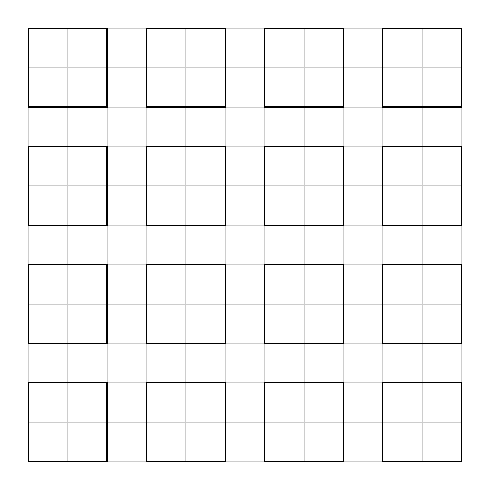
\begin{tikzpicture}
			\draw[step=0.5,very thin,black!20] (0,0) grid (5.5,5.5);
			\path[draw] (0,0)--(1,0)--(1,1)--(0,1)--cycle;
			\path[draw] (0,1.5)--(1,1.5)--(1,2.5)--(0,2.5)--cycle;
			\path[draw] (0,3)--(1,3)--(1,4)--(0,4)--cycle;
			\path[draw] (0,4.5)--(1,4.5)--(1,5.5)--(0,5.5)--cycle;
			\path[draw] (1.5,0)--(2.5,0)--(2.5,1)--(1.5,1)--cycle;
			\path[draw] (1.5,1.5)--(2.5,1.5)--(2.5,2.5)--(1.5,2.5)--cycle;
			\path[draw] (1.5,3)--(2.5,3)--(2.5,4)--(1.5,4)--cycle;
			\path[draw] (1.5,4.5)--(2.5,4.5)--(2.5,5.5)--(1.5,5.5)--cycle;
			\path[draw] (3,0)--(4,0)--(4,1)--(3,1)--cycle;
			\path[draw] (3,1.5)--(4,1.5)--(4,2.5)--(3,2.5)--cycle;
			\path[draw] (3,3)--(4,3)--(4,4)--(3,4)--cycle;
			\path[draw] (3,4.5)--(4,4.5)--(4,5.5)--(3,5.5)--cycle;
			\path[draw] (4.5,0)--(5.5,0)--(5.5,1)--(4.5,1)--cycle;
			\path[draw] (4.5,1.5)--(5.5,1.5)--(5.5,2.5)--(4.5,2.5)--cycle;
			\path[draw] (4.5,3)--(5.5,3)--(5.5,4)--(4.5,4)--cycle;
			\path[draw] (4.5,4.5)--(5.5,4.5)--(5.5,5.5)--(4.5,5.5)--cycle;
		\end{tikzpicture}
		\caption{16 квадратов $2\times2$ на доске $11\times11$}\label{squares}
	\end{minipage}
\end{figure}

\z Из чисел от 1 до 200 выбрано 101 число. Докажите, что среди них можно выбрать два так, чтобы одно делилось на другое.

\s Разделим все числа на 100 кучек. В первую положим $1, 2, 4, 8, \ldots, 128$, во вторую --- $3, 6, 12, \ldots, 192$, в $k$-тую числа вида $(2k-1)\cdot2^i$. Из 101 числа какие-то два будут в одной кучке, а в одной кучке из любых двух чисел одно на другое делится.\QEDA\\

\z В колбе находится колония из 2019 бактерий. В какой-то момент внутрь колбы попадает вирус. В первую минуту вирус уничтожает одну бактерию, и сразу же после этого и вирус, и оставшиеся бактерии делятся пополам. Во вторую минуту новые два вируса уничтожают две
бактерии, а затем и вирусы, и оставшиеся бактерии снова делятся пополам, и т.д. Наступит ли такой момент времени, когда не останется ни одной бактерии?

\s Рассмотрим отношение числа бактерий к числу вирусов. Вначале оно 2019, когда вирусы убивают бактерии, уменьшается на 1, а когда вирусы и бактерии делятся, не меняется. Значит, каждую минуту оно уменьшается на 1 и через 2019 минут станет равно 0.\QEDA\\

\z Коля и Витя играют в следующую игру. На столе лежит куча из 31 камня. Мальчики делают ходы поочерёдно, а начинает Коля. Делая ход, играющий делит каждую кучку, в которой больше одного камня, на две меньшие кучки. Выигрывает тот, кто после своего хода оставляет кучки по одному камню в каждой. Сможет ли Коля сделать так, чтобы выиграть при любой игре Вити? 

\s Коля не сможет этого сделать. Если размер какой-то кучки равен $2^k-1$ для какого-то $k$, то как бы мы ни разделили эту кучку на две, размер большей из кучек не станет равным $2^l-1$. С другой стороны, если это не так, то можно разделить на две кучки, большая из которых $2^k-1$. В самом деле, если в кучке от $2^k$ до $2^{k+1}-2$ камней включительно, то можно выделить кучку с $2^k-1$ камнями и она будет больше, чем другая. Теперь посмотрим на размер максимальной кучки. Изначально он 31, и игра закончится, когда он станет равным 1. Тогда по доказанному ранее Витя сможет играть так, что перед ходом Коли этот размер будет равен $2^k-1$: например, большие кучки делить на кучку $2^k-1$ и меньшую, а все остальные на кучки не больше $2^k-1$. Тогда в тот момент, когда он станет равен 1, будет ход Коли.\QEDA

\end{document}
